% interacttfosample.tex
% v1.05 - August 2017

\documentclass[]{interact}
\usepackage[version=3]{mhchem}
\usepackage{breqn}
\usepackage{amsmath}
\usepackage{graphicx}
\graphicspath{{Figs/}}
\usepackage{mathrsfs}
\usepackage{epstopdf}% To incorporate .eps illustrations using PDFLaTeX, etc.
\usepackage[caption=false]{subfig}% Support for small, `sub' figures and tables
%\usepackage[nolists,tablesfirst]{endfloat}% To `separate' figures and tables from text if required

%\usepackage[doublespacing]{setspace}% To produce a `double spaced' document if required
%\setlength\parindent{24pt}% To increase paragraph indentation when line spacing is doubled
%\setlength\bibindent{2em}% To increase hanging indent in bibliography when line spacing is doubled

\usepackage[numbers,sort&compress,merge]{natbib}% Citation support using natbib.sty
\bibpunct[, ]{[}{]}{,}{n}{,}{,}% Citation support using natbib.sty
\renewcommand\bibfont{\fontsize{10}{12}\selectfont}% Bibliography support using natbib.sty
\theoremstyle{plain}% Theorem-like structures provided by amsthm.sty
\newtheorem{theorem}{Theorem}[section]
\newtheorem{lemma}[theorem]{Lemma}
\newtheorem{corollary}[theorem]{Corollary}
\newtheorem{proposition}[theorem]{Proposition}
\theoremstyle{definition}
\newtheorem{definition}[theorem]{Definition}
\newtheorem{example}[theorem]{Example}
\theoremstyle{remark}
\newtheorem{remark}{Remark}
\newtheorem{notation}{Notation}



\begin{document}

\articletype{ARTICLE TEMPLATE}

\title{UV-induced radicals in $\alpha$-keratin}


\author{
\name{Nadia Babaei Bidmeshki\textsuperscript{a}\thanks{CONTACT Nadia Babaei Bidmeshki. Email: nadia.babaei.2010@gmail.com}, Yavar T. Azar\textsuperscript{b} and Farhood Ziaie\textsuperscript{a}}
\affil{\textsuperscript{a} Radiation Application Research School, Nuclear Science and Technology Research Institute, Tehran, Iran; \textsuperscript{b} Physics and Accelerator Research School, Nuclear Science and Technology Research Institute, Tehran, Iran.}}


\maketitle

\begin{abstract}
This template is for authors who are preparing a manuscript for a Taylor \& Francis journal using the \LaTeX\ document preparation system and the \texttt{interact} class file, which is available via selected journals' home pages on the Taylor \& Francis website.
\end{abstract}

\begin{keywords}
radical; EPR; TDDFT; tables; mathematics; fonts; references; appendices
\end{keywords}


\section{Introduction}


Extended applications of radiation and radioactive materials have led to various incidents in which individuals have absorbed unknown doses of radiation. Among the most well-documented accidents are over-exposure of patients in radiotherapy, the release of radioactive materials in the environment, nuclear reactor accidents, nuclear weapon tests, and nuclear waste mismanagement. One of the most reliable methods in estimating the accidental exposure of individuals is retrospective dosimetry, \cite{OpticalStimulated} in which biologic tissues such as tooth enamel and fingernail are used as dosimeters.



Hair is composed of heavily melanized keratin fibers.
Keratin is insoluble protein complex that forms 65\% to 95\% of hair fiber volume. It is consisted of amino acids bounded with all sorts of bounds (amid, disulfide, hydrogen, ionic and hydrophobic). Amid bounds are strongest and they can be broken only by impact of very strong acids and alkalis or by cutting. Once broken, they can never be restored. Central part of the hair (medulla) is surrounded with cortex – the greatest mass of the hair shaft.
The melanin granules are located inside the cortex and constitute 3\% of hair fiber volume. There are two types of melanin: eumelanin (dark-brown pigment) and pheomelanin (red pigment). Type, size, amount and distribution of melanin granules inside the cortex as well as thickness of hair shaft and content of air in hair shaft, establish hair color. Cortex is surrounded with cuticle, protective layer of overlapping keratinized scales that constitute 10\% of hair fiber volume. Cells of cortex and
cuticle are bonded with structural lipids. Hair shaft is also consisted of other proteins and minerals \cite{sebetic2008}. 


Hair melanins provide some photochemical protection to hair proteins, especially at lower wavelengths, where both the pigments and the proteins absorb light, by absorbing and filtering the impinging radiation and subsequently dissipating this energy as heat. Their high absorption capacity can be explained in terms of their extensive system of conjugate carbonyl groups and double bonds. This not only captures a large fraction of the radiation but also immobilizes many of the free radicals formed upon the absorption of the UV radiation
photo-sensitive amino acids in hair, preventing the transport of these free radicals into the keratin matrix \cite{SantosNogueira2004}.




Fingernails are mainly composed of \(\alpha\)-keratin, a fibrous protein typically high in alanine, leucine, arginine, and cysteine, in which three right-handed helical peptide chains are twisted into a left-handed coil, and they are strengthened by disulfide cross-links \cite{CoiledCoils}. \(\alpha\)-keratin contains large amounts of the sulfur-containing amino acid cysteine, which is required for the disulfide bridges and gives additional rigidity to the structure. Bonding between two active sulfurs leads to the formation of cystine molecule.  This particular bond is firm, and its concentration in hair and fingernails is a determining parameter to control the flexibility and overall shape of these tissues \cite{KeratinStructure, marciniak2016epr}.


Changes due to ionizing radiation in fingernails can serve as the basis of biodosimetry in humans exposed to ionizing radiation \cite{EPRofNail, KeratinStructure, Trompier2014}. Electron paramagnetic resonance (EPR) spectroscopy is a significant technique in dosimetry. The potential for using EPR to measure absorbed dose was first recognized and reported by Saakov et al \cite{EPR}. Radicals formed by ionizing radiation are trapped within rigid solids of fingernail, tooth enamel, and hair. Since the amount of formed radicals is directly related to the absorbed dose, EPR technique can be used to measure the unpaierd electrons created in the biosample. EPR is used for long-lived paramagnetic species that are stabilized in the matrix of the samples \cite{Symon1982, EPRbiodosimetry}.


Numerous researchers have investigated the nature of the long-lived radicals trapped in the keratin matrix \cite{Pailthorpe1972ESRACIDS, 1987-SulphurA-keratins, EPRofNail, Black2010ExRadicals, Trompier2014, Tipikin2016PossibleCalculations}. 


Contradictions are found in the literature about the effect of ultraviolet radiation on hair properties, especially about the effect of specific wavelength ranges. Authors generally attribute hair damage to the total ultraviolet range of the solar spectrum and relate the photo-sensibility of light and dark hair to hair melanin type. Ruetsch
et al. \cite{Ruetsch2000} state that the amino acids cystine and methionine are those most degraded by UV radiation. 
Pande and Jachowicz\cite{Pande1993} indicate that UVA and visible radiations do not cause direct damage to hair because they are not absorbed by hair proteins. These authors also mention that tyrosine and tryptophan are the most degraded amino acids after hair exposure to UV radiation.


%%%%%%%%%
Recently it has been suggested,(l)on the basis of UV absorption spectrometry, that tryptophan residue decomposition is mainly responsible for the production of the yellow discolouration although considerable degradation other than this undoubtedly occurs. The purpose of this investigation was to explore further the photolytic effects of UV radiation on keratin using electron spin resonance spectroscopy \cite{Dunlop1965}. The electron spin resonance spectra resulting from the UV irradiation of proteins are
believed to be produced by several different reactions related to the energy absorptions
of the various chromophores present in proteins, particularly those of tryptophan, tyrosine, cystine and phenylalanine. The probable form of this free radical is believed to be
HZN \
CH - CH2 - S.
HOOC/
It was observed that irradiated tyrosine spectrum is similar to that of tryptophan. 

The electron spin resonance spectra of the cystine containing proteins are distinguished by an asymmetric double peak (A and B). This feature of the spectra corresponds quite closely in g-value and hyperfine splitting with the spectra of irradiated cystine, cysteine and glutathione, suggesting that it is produced by a free radical located at the cystine residues. The double peak A and B may not be the only effect of this cystine free radical. It is certain that part of the spectrum around g=2 is also produced by this radical, the remainder being due to the presence of other species of free radical, as indicated by the differences between these spectra and the glutathione spectrum and by differences between the protein spectra themselves. Graphical subtraction of the glutathione spectrum from any of these
protein spectra results in a single line spectrum. This difference spectrum is similar to that of irradiated tyrosine or tryptophan but there are not enough spectral characteristics to allow a positive identification. Thus, it may be
concluded that the cystine containing proteins exhibit electron spin resonance spectra which are compounded of at least two different free radical species-one located on the cystine residue and one or more of unknown origin.

The results of these aeration studies indicate that the formation of free radicals in proteins is more complex than has been suggested by earlier observation. It leaves no doubt, however, that at least two different free radicals are formed by the UV irradiation of keratin.


This study has shown that stable free radicals are produced as intermediates in the
photochemical processes induced by the UV irradiation of proteins. Considerations
of the effects of the wavelength of irradiation have indicated that the free radical production is closely associated with the energy absorptions of the chromophores present in the proteins. Several species of free radicals are produced by the UV irradiations but it has been possible to identify only those free radicals associated with the cystine residues.
A major point of interest to emerge is that the exposure of wool or other forms of keratin to sunlight will result in the formation of free radicals. The free radicals produced by the shorter wavelengths present in sunlight, that is, in the 3000-3250 A range are those associated with the cystine residues, indicating cystine residue decomposition, and others of a less determinate nature. These free radicals are reactive and decay by their combining with air. The longer wavelengths of UV (3250-4000 A) and visible (4000-6000 A) radiation of which there is an abundance in sunlight also lead to the formation of free radicals but of a more stable nature.

%%%%%%%%%%%%%%%%%%%%%%%%%


Comparing both spectra, we observe that
keratin absorbs mainly UVB radiation and that melanin absorbs UVB, UVA and visible radiations. \cite{Santos2004}


%%%%%%%%%%%%%%%%%%

UV radiation induces the formation of oxyradicals such as superoxide (\ce{O_2^{.-}}), and hydroxyl (\ce{OH^{•}} ). These species have one unpaired electron in an outer orbital giving them a very powerful aptitude to react, especially with molecules having a double bond in their structure, such as unsaturated lipids. Chemically, these changes are thought to be caused by UV light-induced oxidation of the sulfur-containing molecules within the hair shaft. Melanin has an intrinsic electron spin resonance (ESR) signal that increases significantly when irradiated with UV-visible light. In the presence of oxygen, superoxide is produced, which dismutates to hydrogen peroxide. This leads to the formation of hydroxyl radicals in the presence of trace amounts of metal ions. Oxidation of the amide carbon of polypeptide chains also occurs, producing carbonyl groups. \cite{Nogueira2006}

Davidson33 reviewed the photochemistry of wool keratin. Similarly to human hair, the most apparent damages caused by ultraviolet and visible radiation are a color change and a weakening of the fiber. Depending on the spectral distribution of the sunlight, it either yellows or bleaches. Wool keratin also contains significant amounts of the aromatic amino acids, tryptophan, tyrosine and phenylalanine. These amino acids are the major chromophores in wool in the spectral range 250–310 nm and as such they are expected to play a significant part in its photodegradation upon exposure to sunlight. Furthermore, this etiesfiber also loses its strength and bleaches at longer wavelengths, showing that these chromophores are photochemically active and important in the photodegradation of the protein. Most of these species are probably either thermal decomposition or photolysis products of the constituent amino acids of keratin. Free radicals have been observed by ESR spectrometry during the light-induced degradation of keratin. Carbon-centered radicals are formed with an action spectrum maximum of 285 nm, suggesting that they are primary photoproducts of aromatic amino acids.34 Kinetics measurements indicate that there are at least three types of radicals produced at this wavelength. Stable sulfur-centered radicals are formed from irradiation of dry keratin in the absence of oxygen, but their ESR signals disappear in the presence of moist air. The presence of small amounts of metal ion induce the production of free radicals from irradiated keratin at wavelengths above 320 nm, apparently due to the formation of metal–protein complexes that absorb at higher wavelengths.35



%%%%%%%%%%%%%%%%%%%

All adverse external impacts that are causing degeneration of hair are called weathering by Rook and his associates. Excessive sun exposition is the most frequent cause of hair shaft’s structural impairment. Dryness, reduced strength, rough surface texture, loss of color, decreased lustre, stiffness and brittleness of hair are caused by sun exposure3. UVB radiation maintains in cuticle area, while UVA radiation passes through cuticle and penetrates to cortex. Photochemical impairment of the hair includes degradation and loss of hair proteins as well as degradation of hair pigment. Hair protein degradation is induced by wavelengths of 254–400 nm2. UVB radiation is responsible for hair protein loss and UVA radiation is responsible for color changes2,3. Amino acids cystine, methionine, tryptophan, tyrosine and histidine are the most submissive to photochemical degradation.
Ultraviolet radiation is causing oxidation of afore-mentioned amino acids as well as oxidation of the amid carbon of polypeptide chains4. These reactions are giving yellowish tone to the hair, which is called photoyellowing5. The amino acids of the cuticle are altered to a greater extent than those of the cortex because the outer layers of the fiber receive higher intensities of radiation5. This exposure can cause rupture and detachment of the external layers resulting in splitting of the ends. Portion of certain amino acids depends on the type of hair. Dark and black hair has more photosensitive amino acids (for example cystine) than fair hair2,5. Therefore dark and black hair has the biggest protein loss in the cuticle area.
Increased exposition to sunlight also causes disappearance of lipids and cuticular layer, which contributes to hair changes. UVB radiation causes superficial micro structural changes of cuticle. Such damaged protective
layer of hair shaft enables further degradation processes.
Those impairments are even more expressed in conditions of very enhanced or decreased humidity. Melanin absorbs and filters adverse UV radiations (UVA and UVB) and subsequently dissipates this energy as heat2,5. Therefore it protects hair proteins. However absorption
of radiation in photosensitive amino acids of the hair and their photochemical degradation is producing free radicals. They have adverse impact on hair proteins, especially keratin. Melanin can partially immobilize free radicals and block their entrance in keratin matrix2. Therefore melanin is important for direct and indirect protection of hair proteins. In described processes of photo protection melanin fades. Opinions about photo stability of feomelanin and eumelanin (resistance of dark and faire hair towards UV radiation) are divided6. Some authors are considering dark hair to be more resistant to photo degradation regarding to larger photo stability of eumelanin. On the other side there are opinions of less degradable pheomelanin. Anyway it seems that resistance of dark and faire hair to photo oxidation is not related to type of melanin but with its quantity. In fact, hair with more pigmented granules shows less protein loss during exposition of UV radiation7,8 \cite{sebetic2008}.
%%%%%%%%%%%%%%%%%%%%%%%%%%%%%%%

Fluorescence and other spectral parameters of aromatic chromophores in proteins, tryptophan, tyrosine (Tyr) and phenylalanine, may be used as probes of protein structure. Using Tyr is an attractive choice because its chromophore, phenol, is expected to exhibit substantial responses to environmental changes. The Tyr chromophore, phenol, is an aromatic compound with the molecular formula C6H5OH, bound to the C$\alpha$ carbon
in Tyr at the para position relative to the hydroxyl group.

Phenol is a derivative of benzene. Absorption (and fluorescence)
spectroscopy of a benzene ring can be used to detect its presence in a larger compound and to probe its environment (Nguyen et al. 2003). Valence $\pi$ $\pi$  excitation of benzene results in three absorption bands in the
180-270 nm region.

In the UV absorption spectrum of phenol in cyclohexane, two bands originating from $\pi$ → $\pi$  transitions are observed (Zhang et al. 2006): a primary band at 210 nm (the 1La band) and a secondary band at 269 nm (the 1Lb band) (Dearden and Forbes 1956). In ethanol, these shift to 218.5 and 271 nm (Dearden and Forbes 1956), as a result of involvement of phenol hydroxyl group in various forms of hydrogen bonding (Coggeshall and Lang 1948). Substituted phenols give similar band positions and intensities as those
observed for phenol.
Figure 4 shows the change in absorption spectrum of p-cresol on transfer from cyclohexane (apolar, no hydrogen bonds with solvent molecules) to methanol (polar, the hydrogen bonds possible). A red shift of the Lb transition of approximately 3 nm can be clearly seen. Moreover, the highly structured vibrational peaks, distinct in the presence of cyclohexane, are not apparent with methanol as the solvent. This is due to hydrogen bonding between p-cresol and methanol.




%%%%%%%%%%%%%%%%%%%%%%%%%%%

Tyrosine and cystine are the most mentioned radicals. How can these make radical? there are many mechanisms that talk about radical formation. one is mentioned in \cite{GROVES2018}




Several reports on the oxidation of tryptophan to kynurenine4 are found in the literature but there have been few studies that investigate specific radical pathways that lead to the measured EPR signal.



There are two processes which influence the observed radical signal in these EPR studies: the rate of radical formation and the rate of further reactions leading ultimately to radical destruction. Manipulating humidity does not significantly impact the rate of radical formation, however it does change the rate of radical destruction reactions. The lower radical concentrations observed at higher humidity are due to more rapid radical decay. Conversely, excluding oxygen does have a significant effect upon the rate radical formation, as shown in Figure 7. Therefore, in the absence of oxygen, hair damage is significantly reduced due to the lower rate of radical formation. The absence of a characteristic sulfur component in the air-free sample spectrum after exposure indicates that oxygen also plays a crucial role in the formation of secondary radical species.

Formation of radical species on aromatic amino acid residues is facilitated through interactions between excited states and oxygen, leading to the formation of reactive oxygen species. Reactive oxygen species facilitate transfer of radical centers, resulting in increased cleavage of disulfides and polypeptide backbone22. For instance, energy transfer from excited state tyrosine can lead to the formation of reactive oxygen species.23 Oxygen can also interact with radical species, leading to the formation of peroxyl radicals. These form hydroperoxides, which break up to yield alkoxyl and hydroxyl radicals.24 Auto-oxidation cycles lead to degradation of amino acid side chains, disulfide bonds and the polypeptide backbone. These processes are summarized in Figure 1.

%%%Fig1
\begin{figure}
	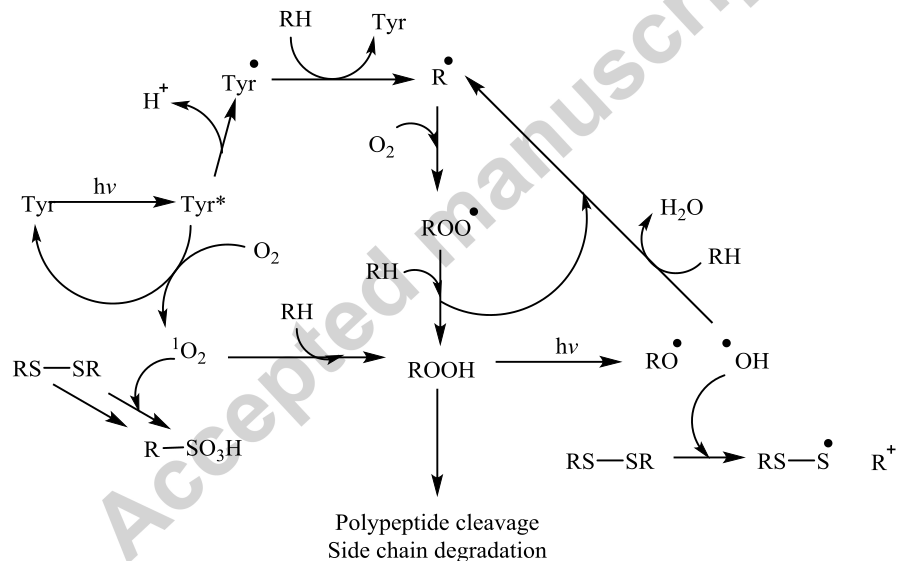
\includegraphics[width=\textwidth]{fig1.png} 
	\caption{Summary of light-induced autoxidation processes leading to polypeptide cleavage, disulfide cleavage and side chain degradation in proteins. R = amino acid side chain or $\alpha$-carbon of amino acid in polypeptide.}
	\label{OxidationProcess}
\end{figure}

%%%%%%%%%%%%%%%%%%%%%%%%%%%%





%%%%%%%%%%%%%%%%%%%%%%%%%%%%%%%

The remainder of the paper is organized as follows: Section II is devoted to explanation of employed computational methods for the model systems studied and the quantum chemical methods used. In Section III, we present our results for spin states and magnetic parameters of model structure emphasizing the role of neighbor residues and environmental effects in tuning the EPR signals. We finally conclude our work in Section IV with a discussion.




\section{Computational Method}
Accetylation and amidation were applied to the terminals of tyrosine. This was done in order to cancel the artifact of the charged terminals.
The optimized structures were subjected to tddft at LC-BLYP/6-31+G(d,p) level of theory \cite{Iikura2001}.
The first excited state was determined.
The structure was optimezed in the first excited state.
And TDDFT was applied to the first excited state. 
The two optimized structures were compared in chemcraft.
The difference between the two cube files of TDDFT simulations were calculated and the charge transfer were detected. 
O-H bond length in two different optimized structures was compared.
Water molecules were insert to the structure to detect whether it is blocker or not.
Electric field effect was investigated.
Quantum chemical EPR/NMR calculations was also done to evaluate $g$-tensor and hyperfine couplings. simulations were carried out by the ORCA package \cite{neese2018software}.


\section{Result and Discussion}
In this section, we are going to analyze the computational and experimental spectra for tyrosine. 



\begin{figure}
	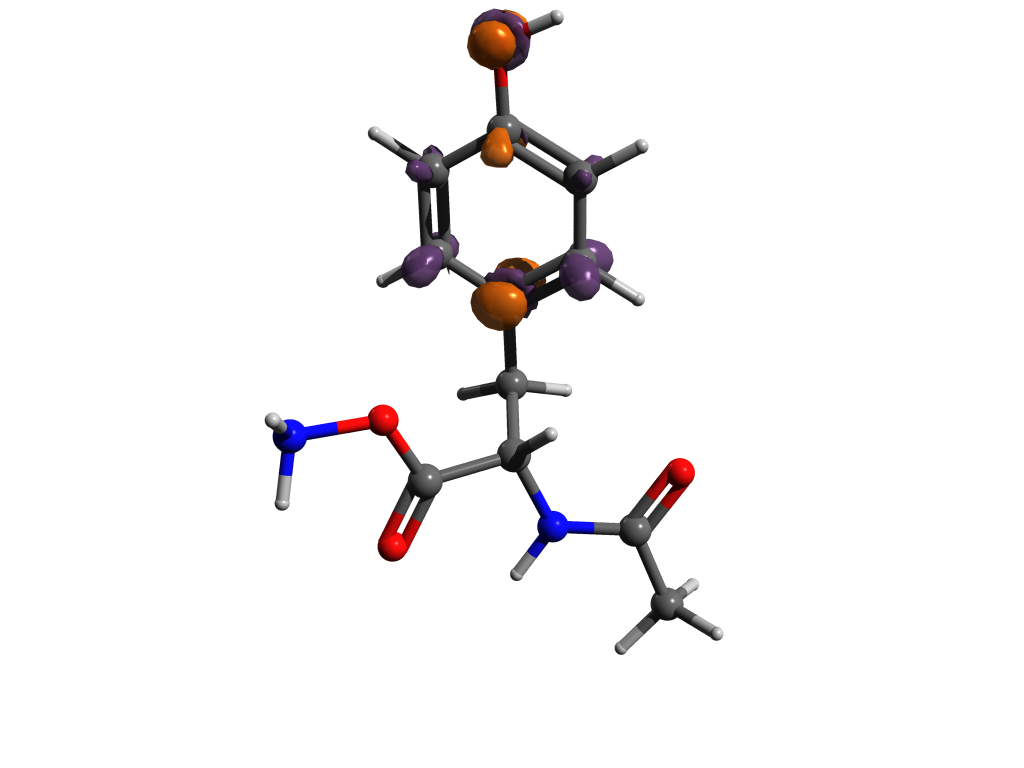
\includegraphics[width=\textwidth]{diff.png} 
	\caption{Cube difference between ground state and first excited state of tyrosine.}
	\label{cubediff}
\end{figure}

\begin{figure}
	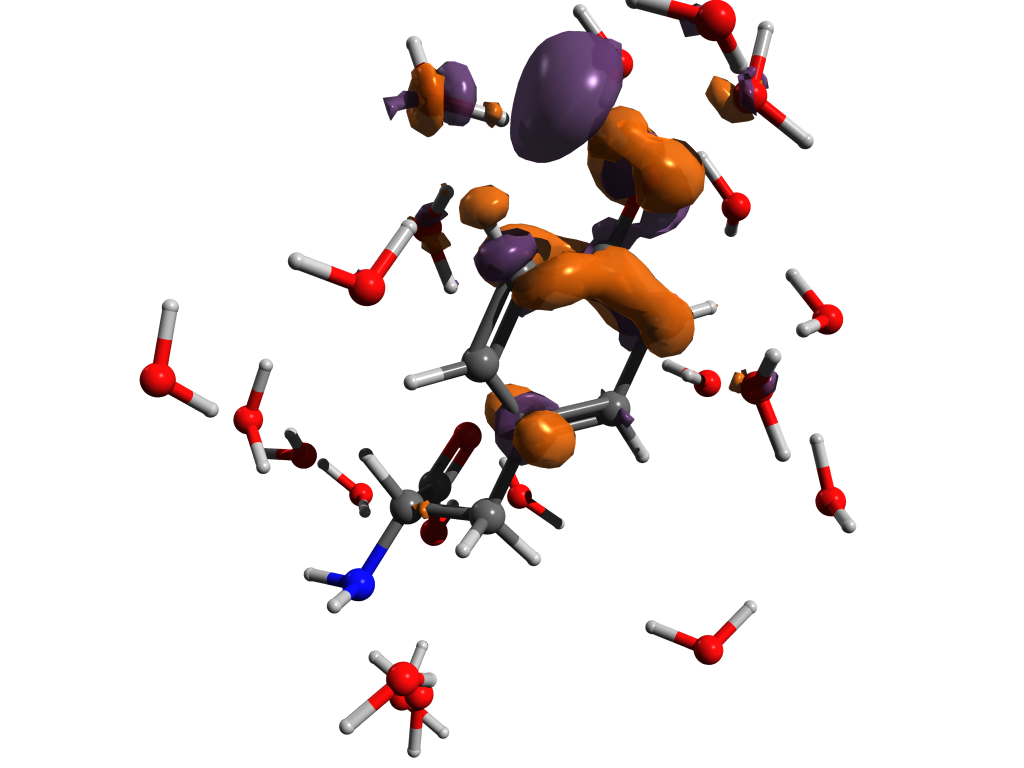
\includegraphics[width=\textwidth]{diffH2O.png} 
	\caption{Cube difference between ground state and first excited state of tyrosine surrounded by water.}
	\label{cubediffH2O}
\end{figure}

\begin{figure}
	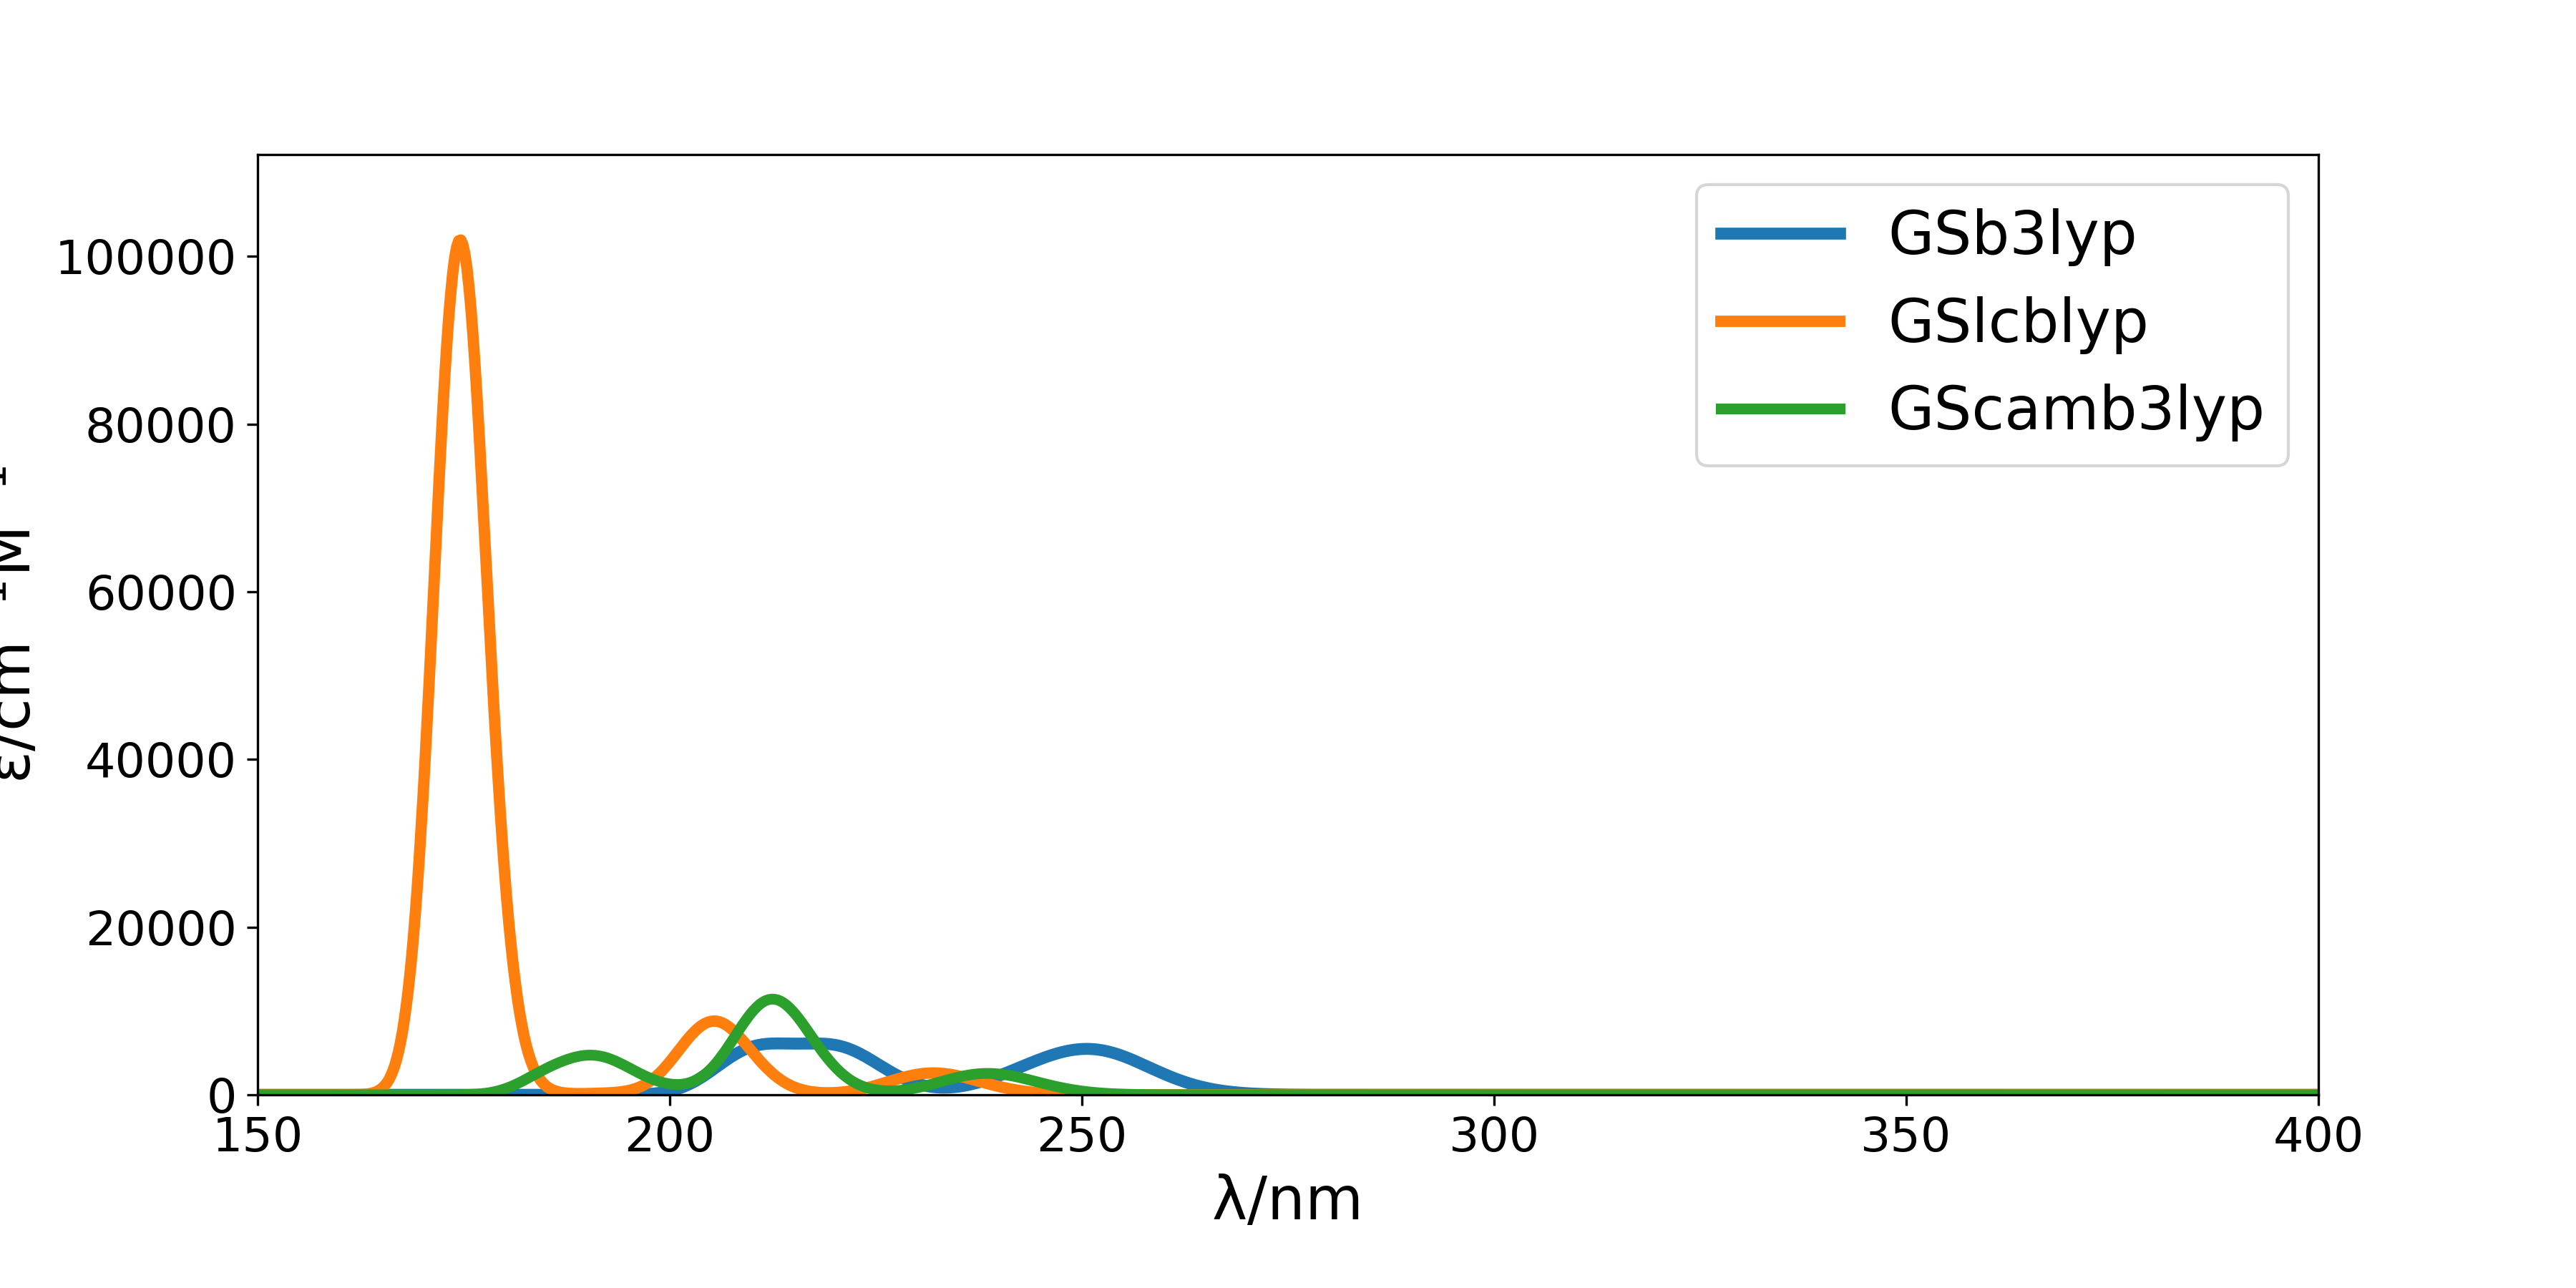
\includegraphics[width=\textwidth]{GS.png} 
	\caption{Comparison of different theory levels in ground state.}
	\label{GSlevel}
\end{figure}

\begin{figure}
	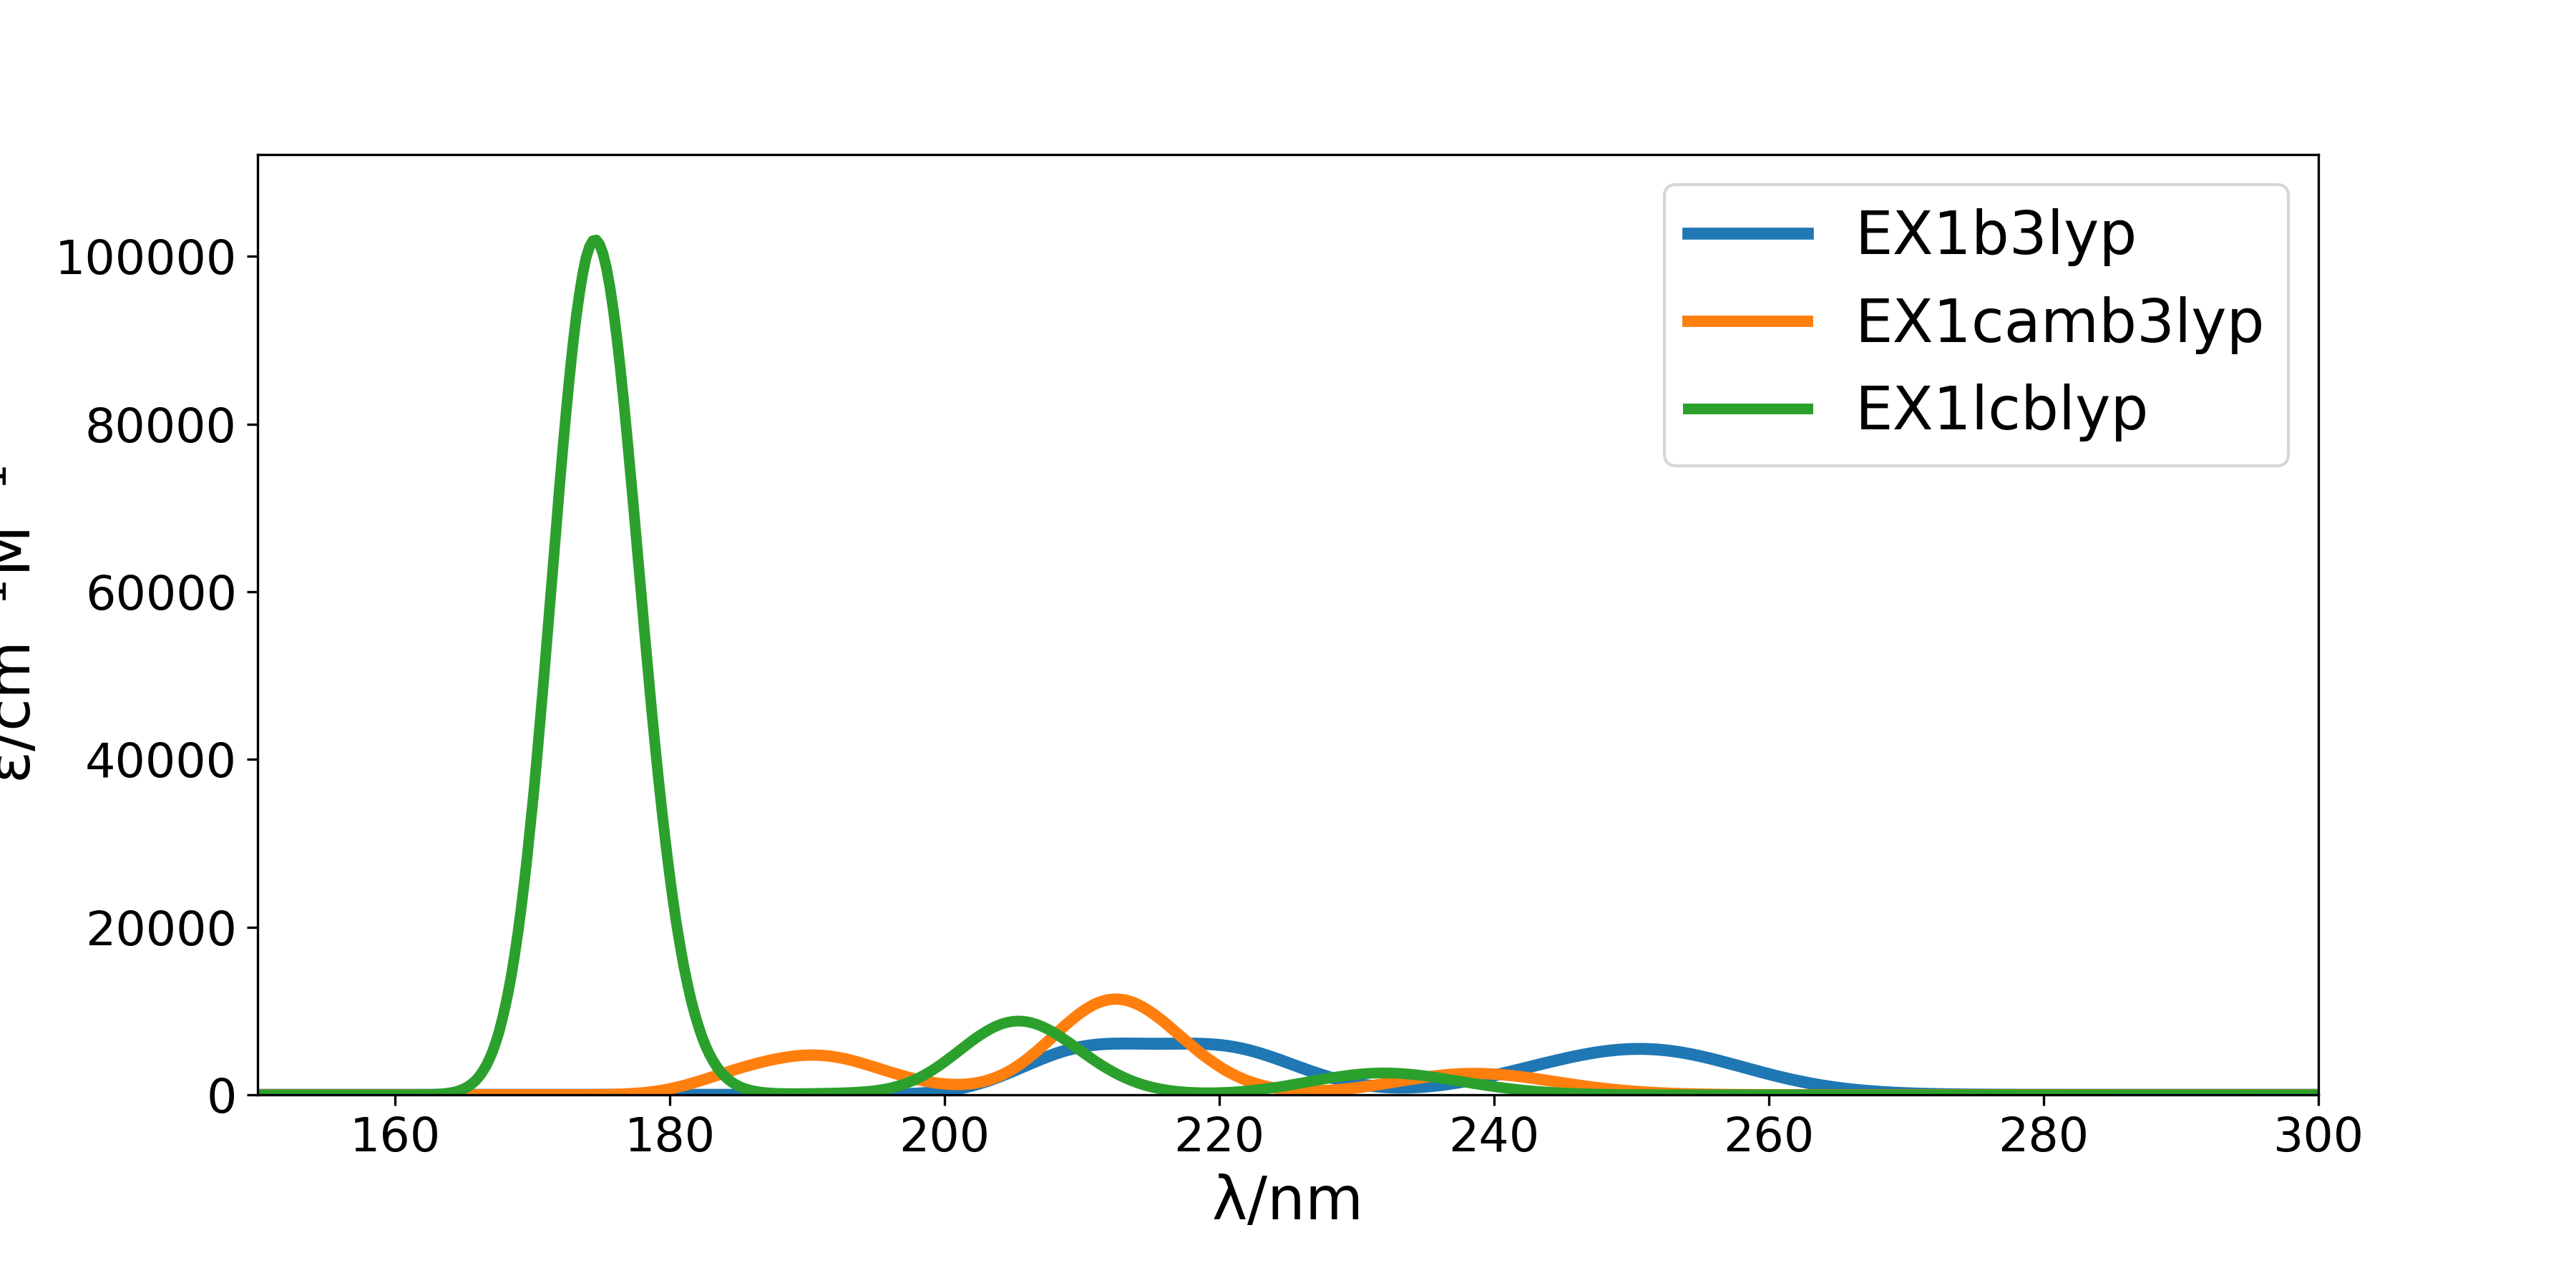
\includegraphics[width=\textwidth]{EX.png} 
	\caption{Comparison of different theory levels in the first excited state.}
	\label{EXlevel}
\end{figure}

\begin{figure}
	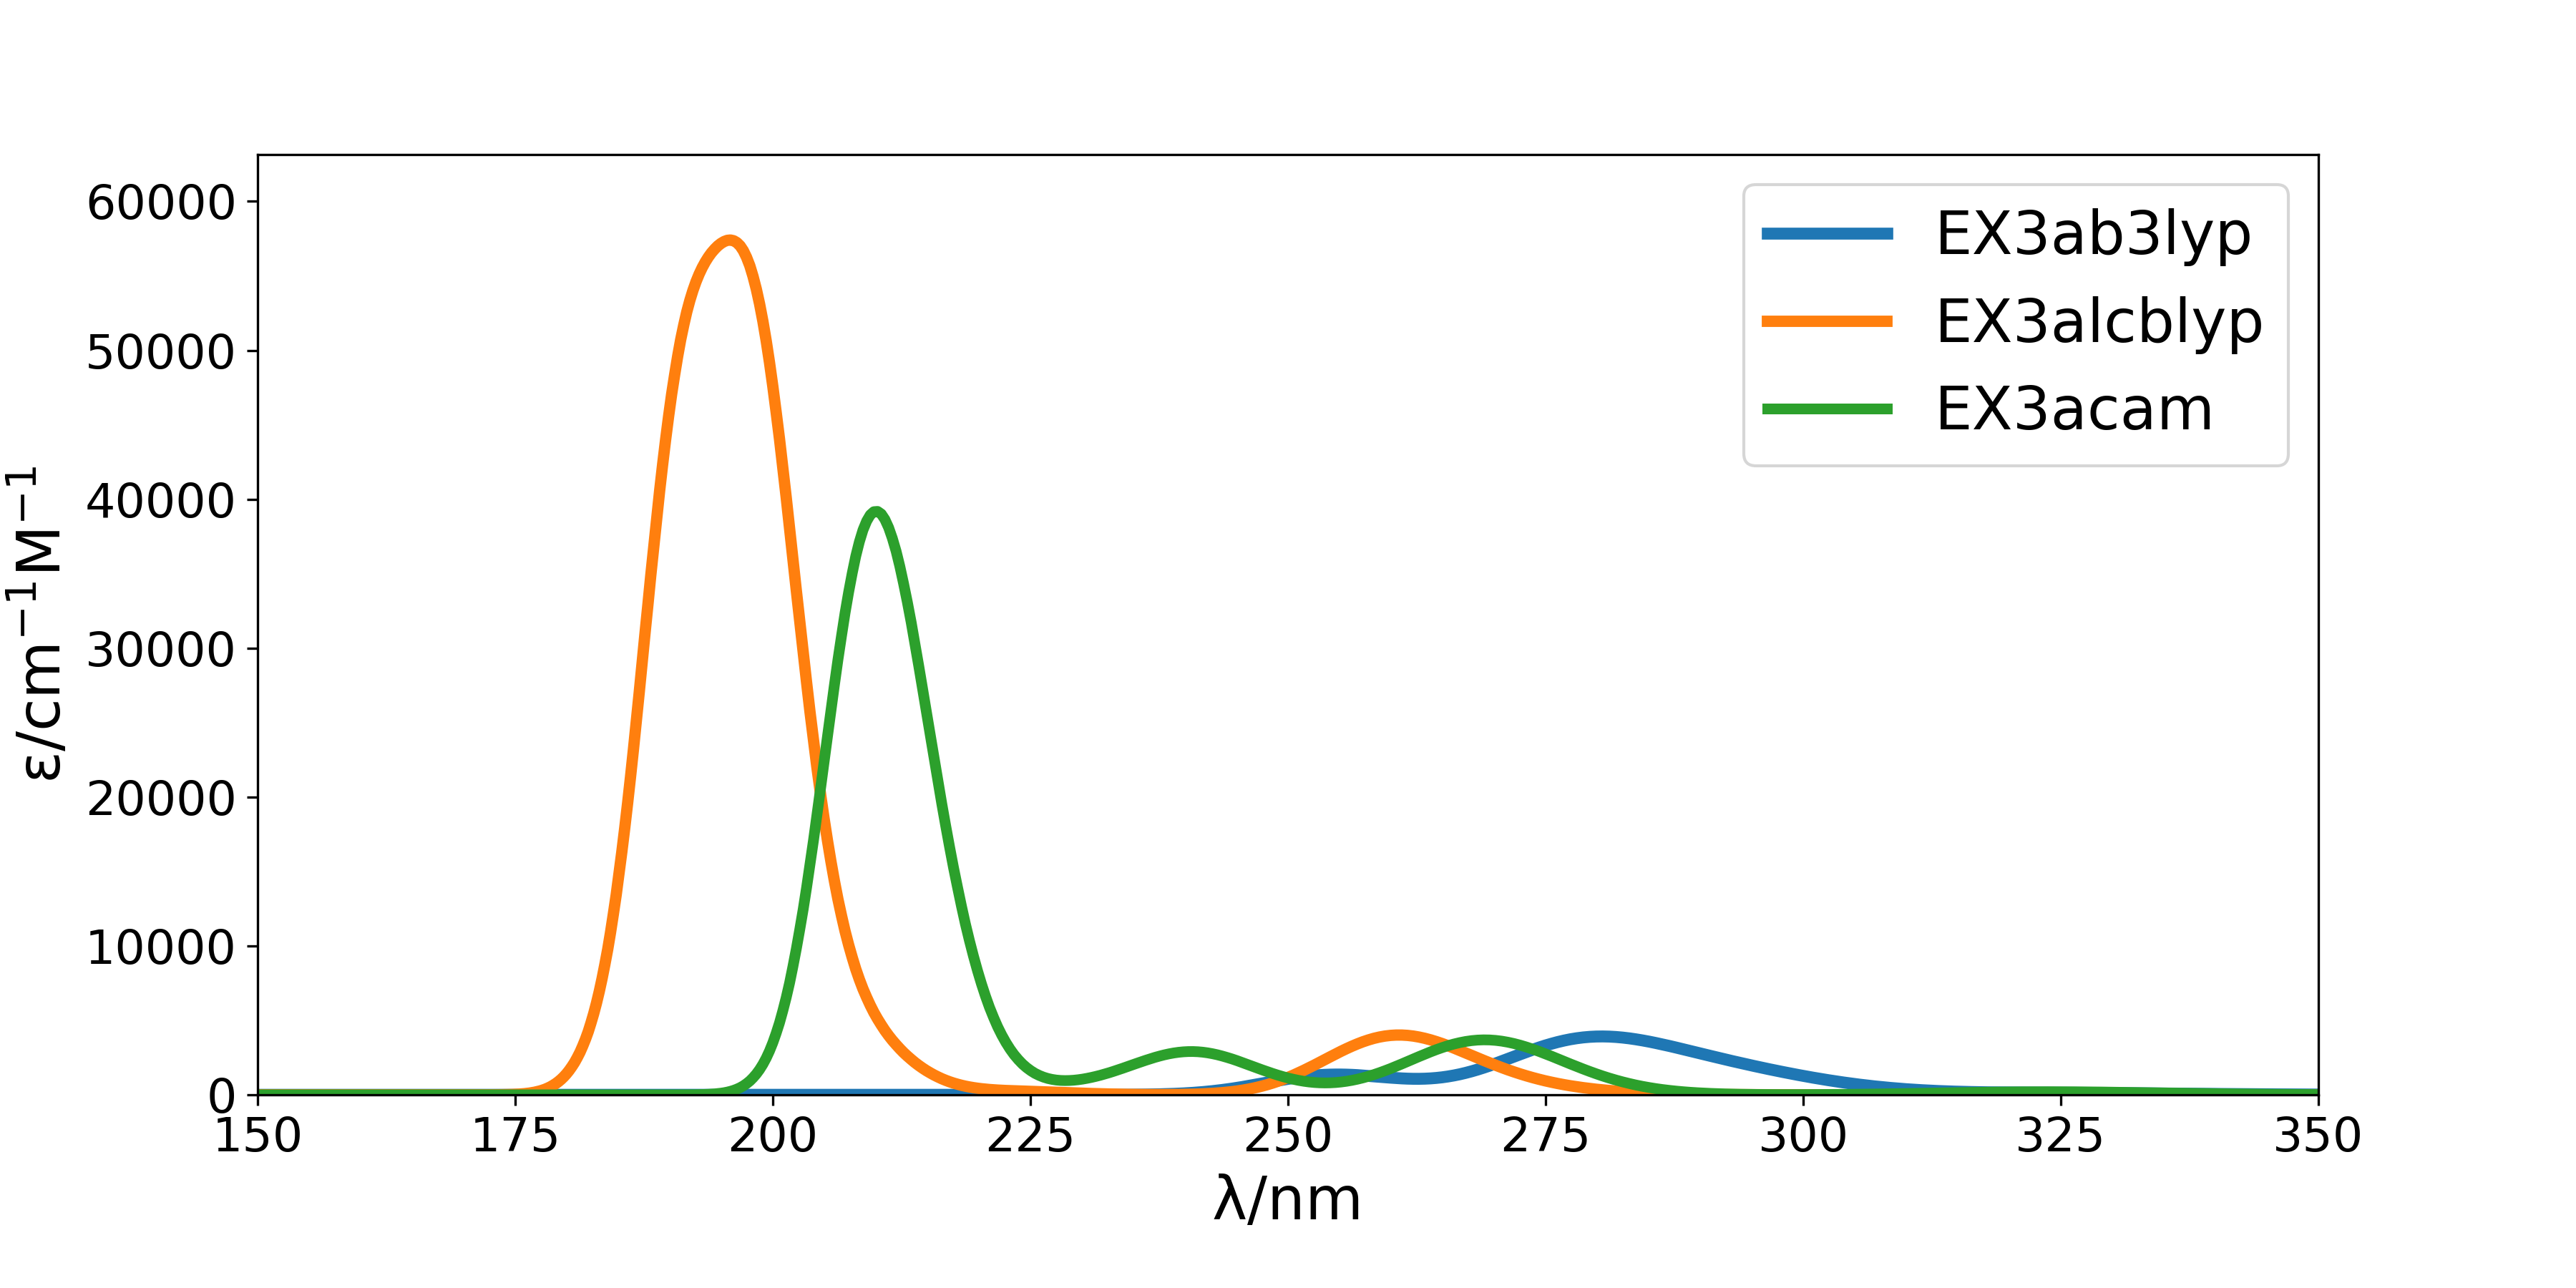
\includegraphics[width=\textwidth]{EXh2o.png} 
	\caption{Comparison of different theory levels in ground state and in explicit environment.}
	\label{EXh2olevel}
\end{figure}

\begin{figure}
	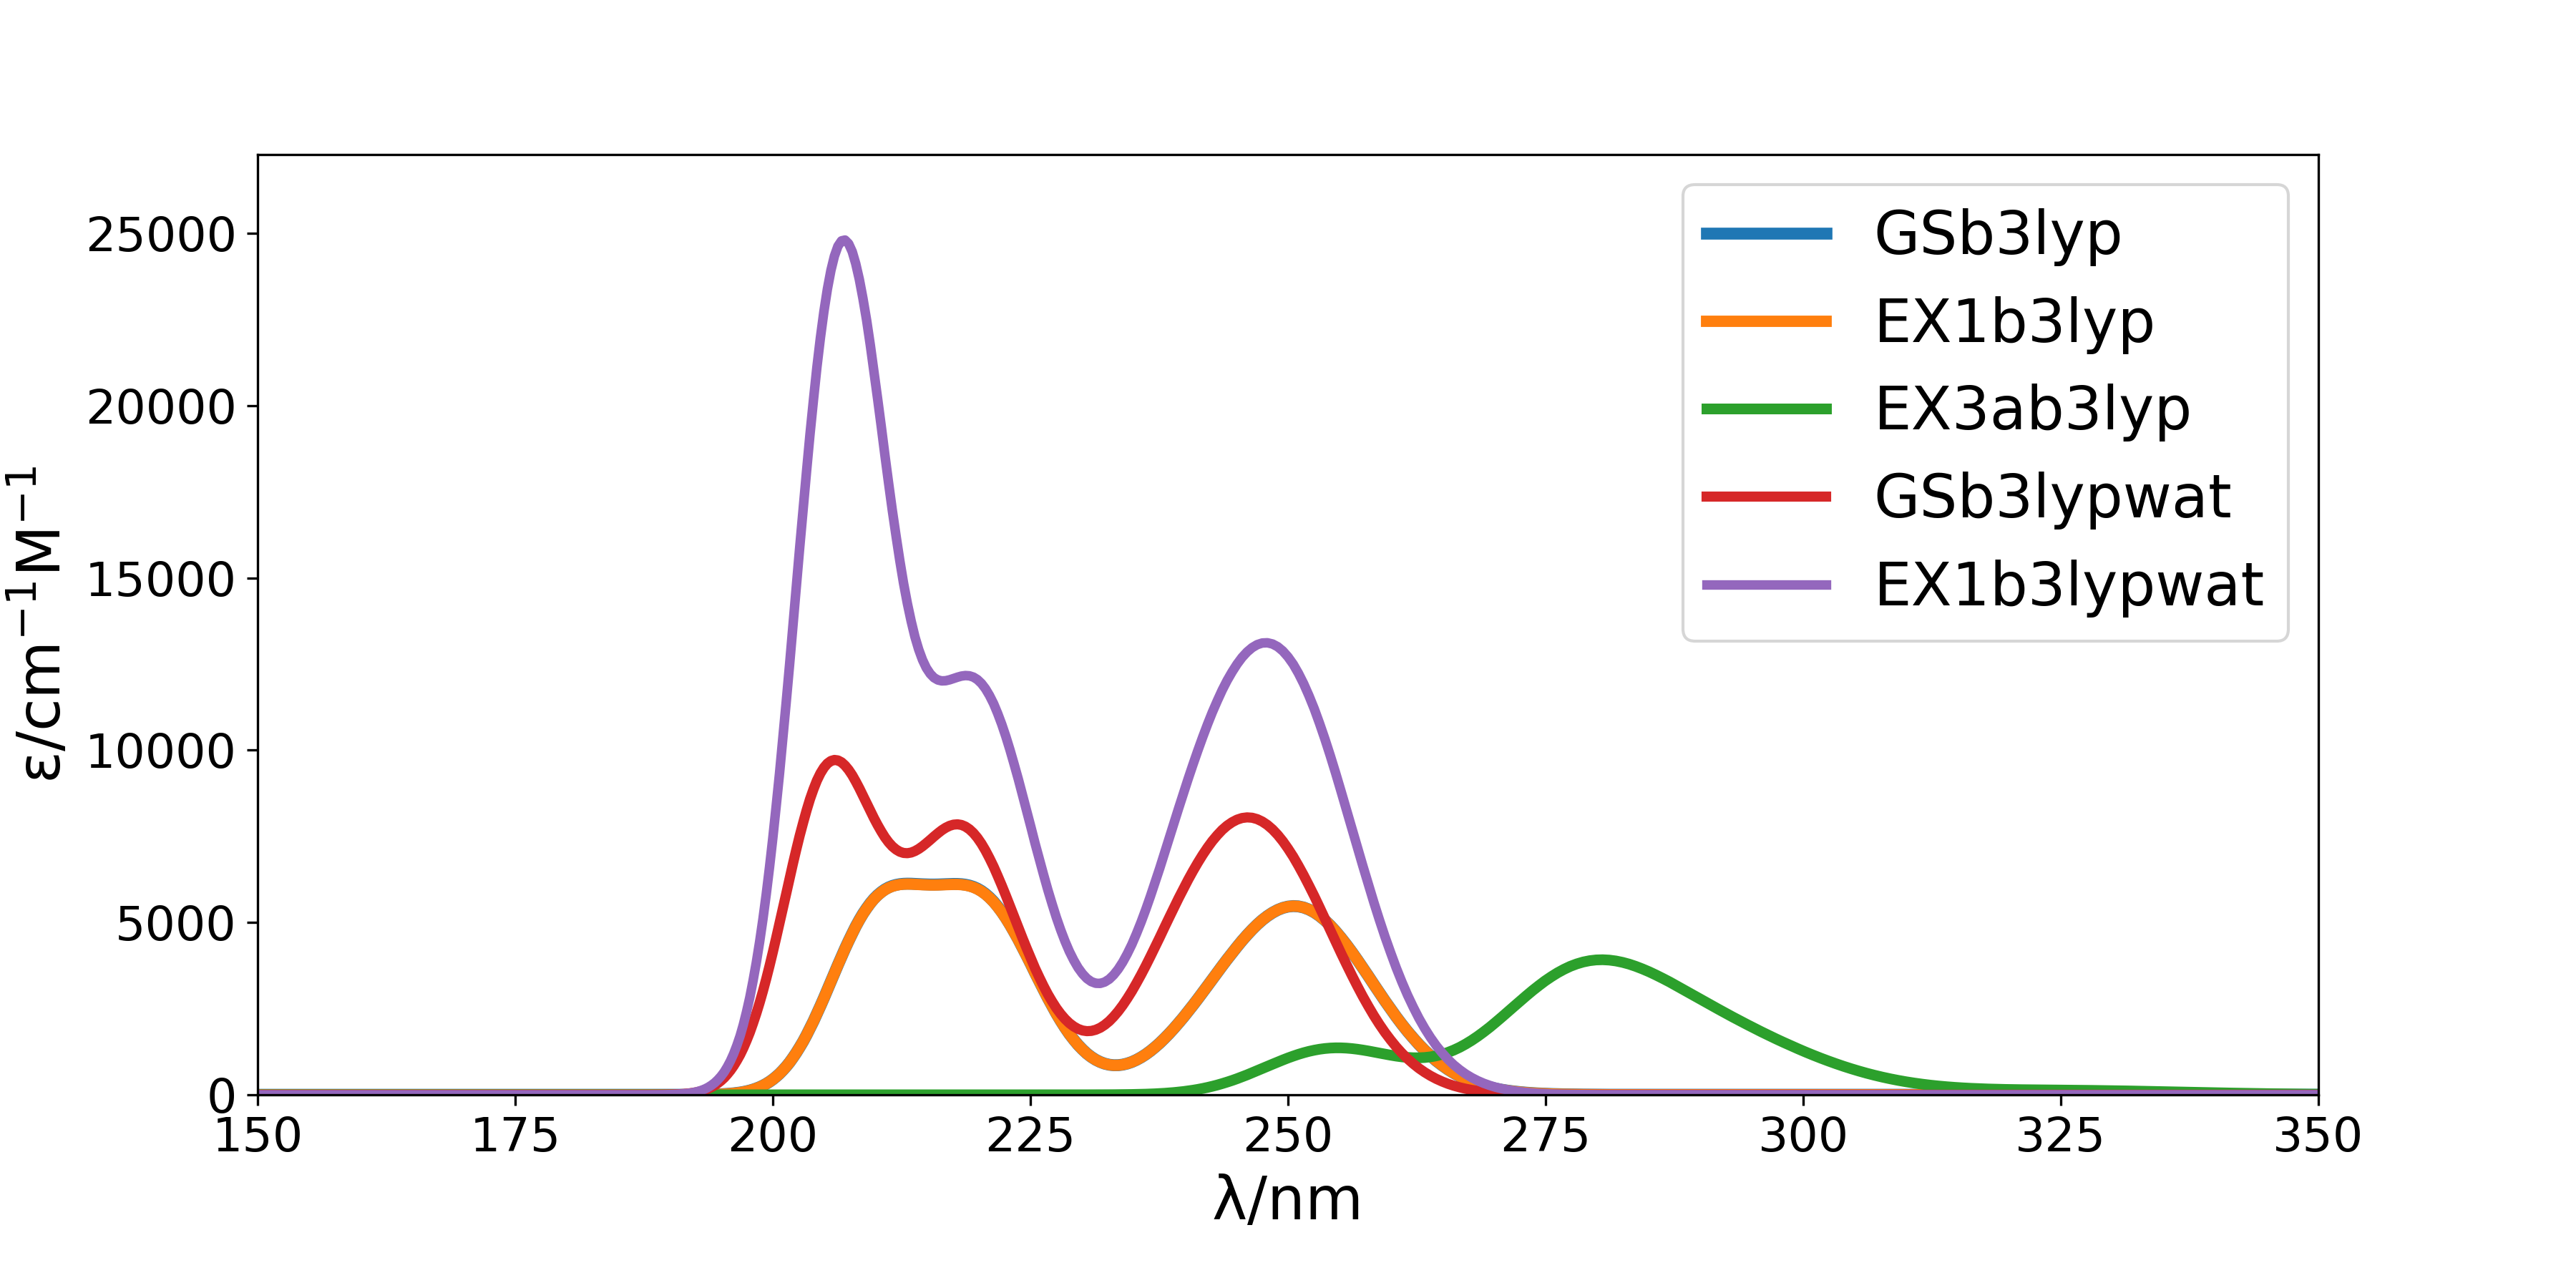
\includegraphics[width=\textwidth]{COMPb3lyp.png} 
	\caption{Comparison of different situations of tyrosine molecule calculated by b3lyp level of theory.}
	\label{COMPb3lyp}
\end{figure}

\begin{figure}
	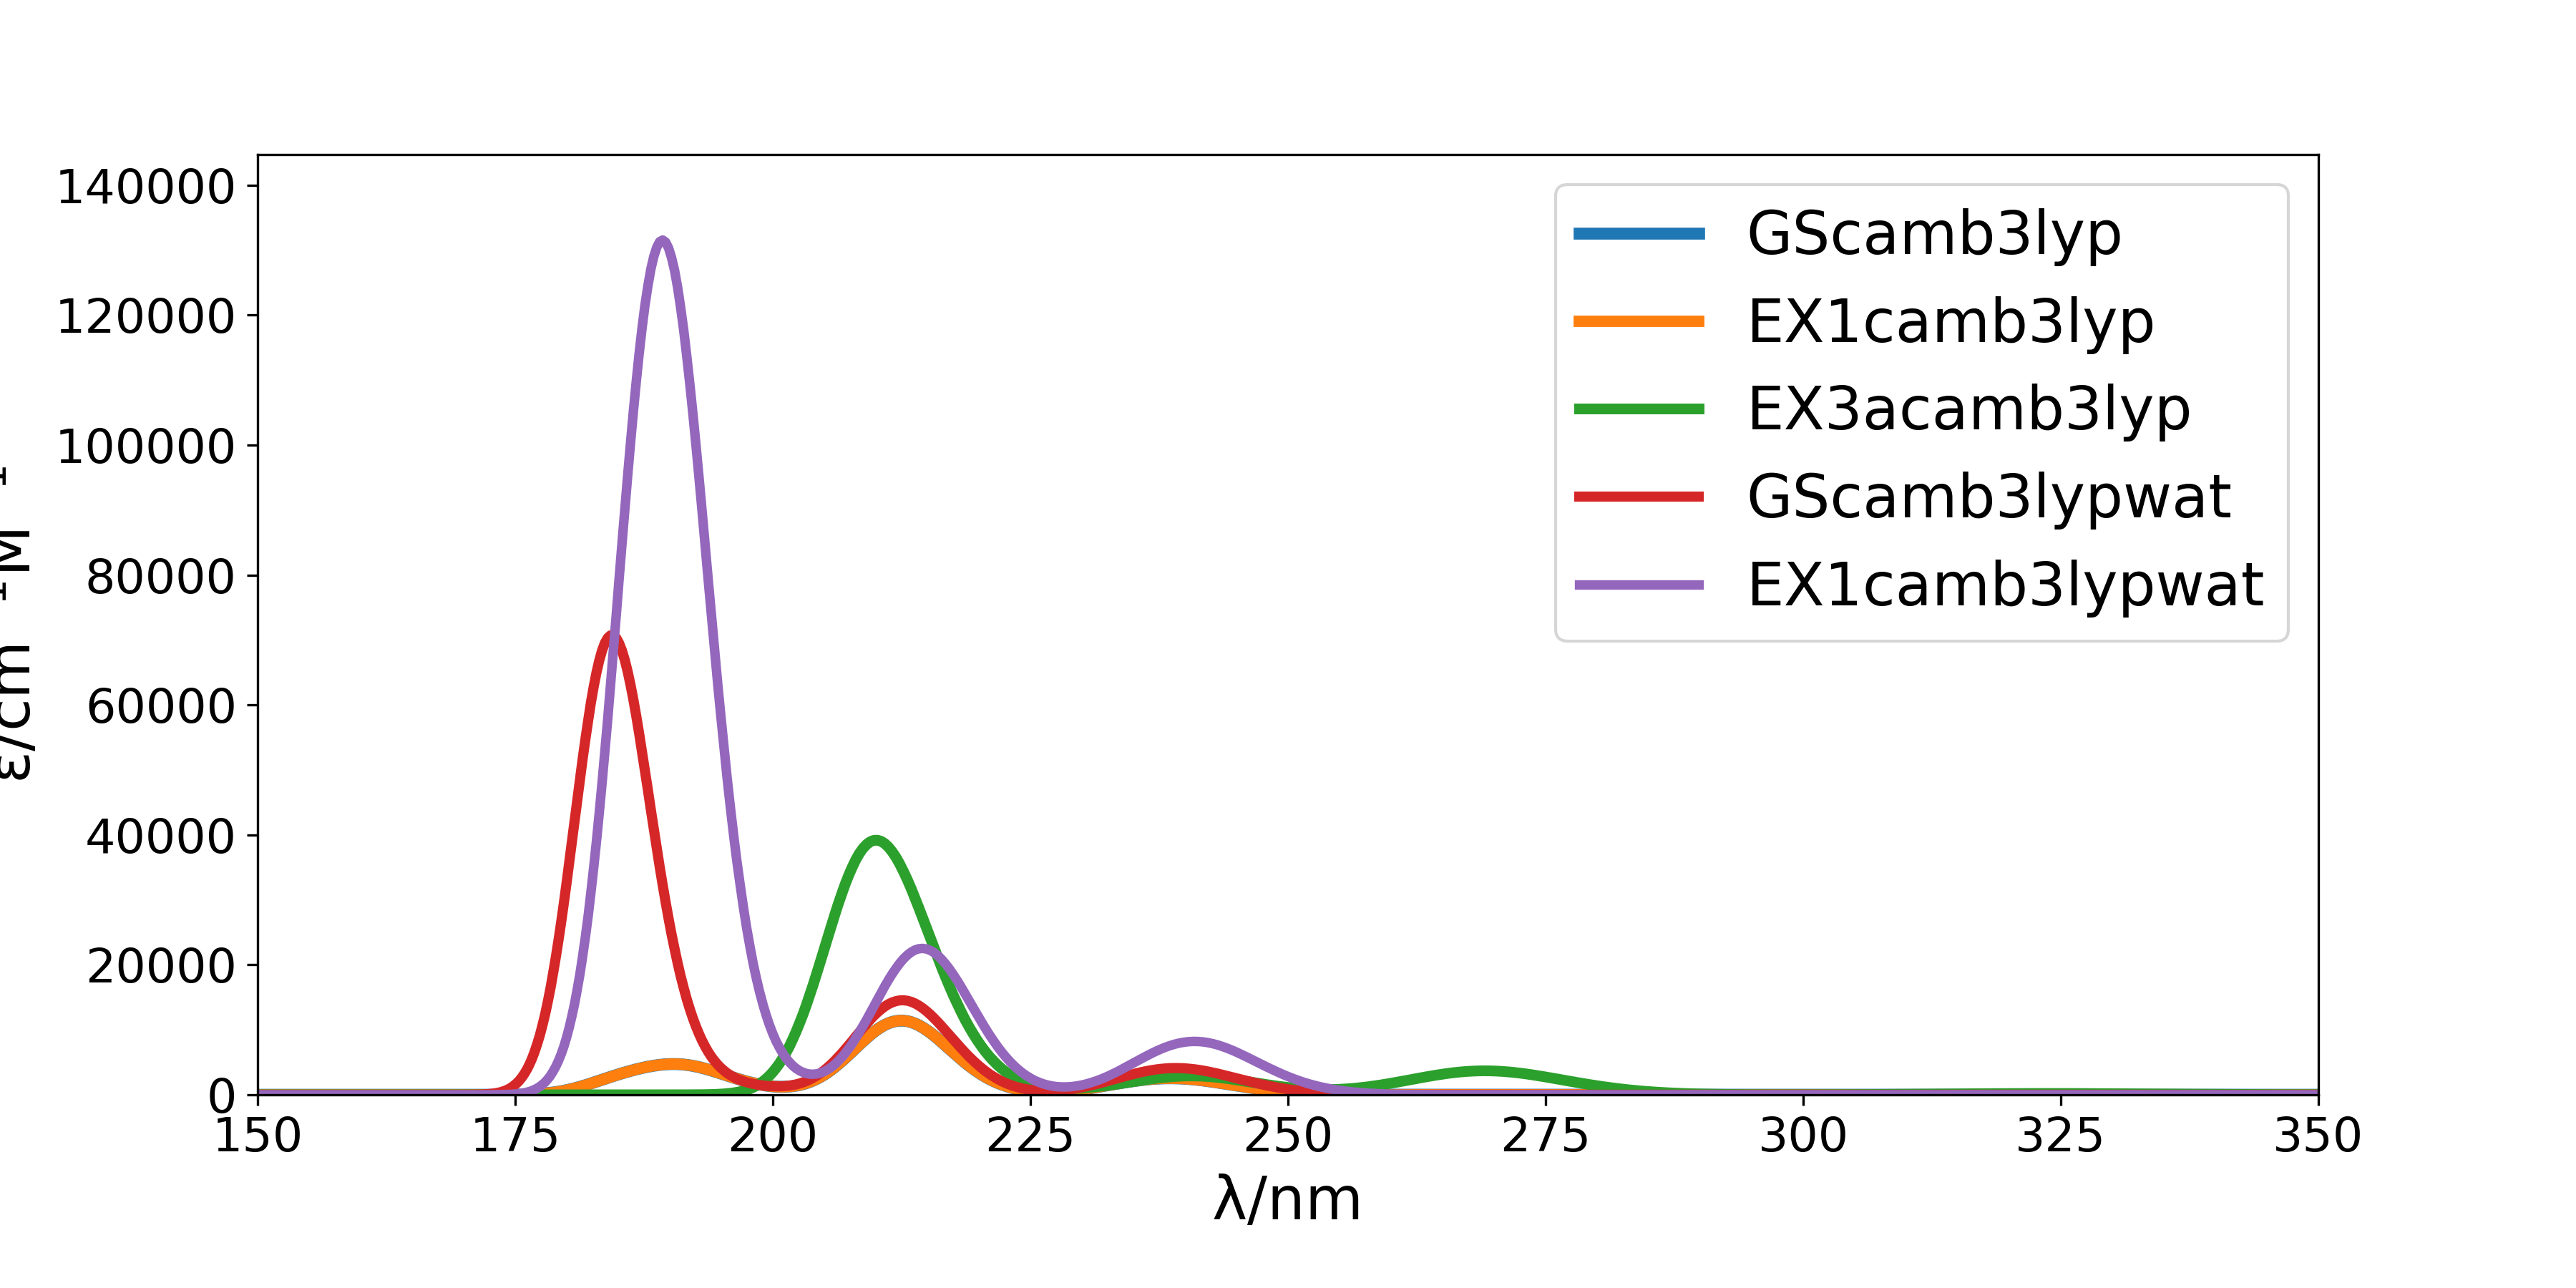
\includegraphics[width=\textwidth]{COMPcamb3lyp.png} 
	\caption{Comparison of different situations of tyrosine molecule calculated by camb3lyp level of theory.}
	\label{COMPcamb3lyp}
\end{figure}

\begin{figure}
	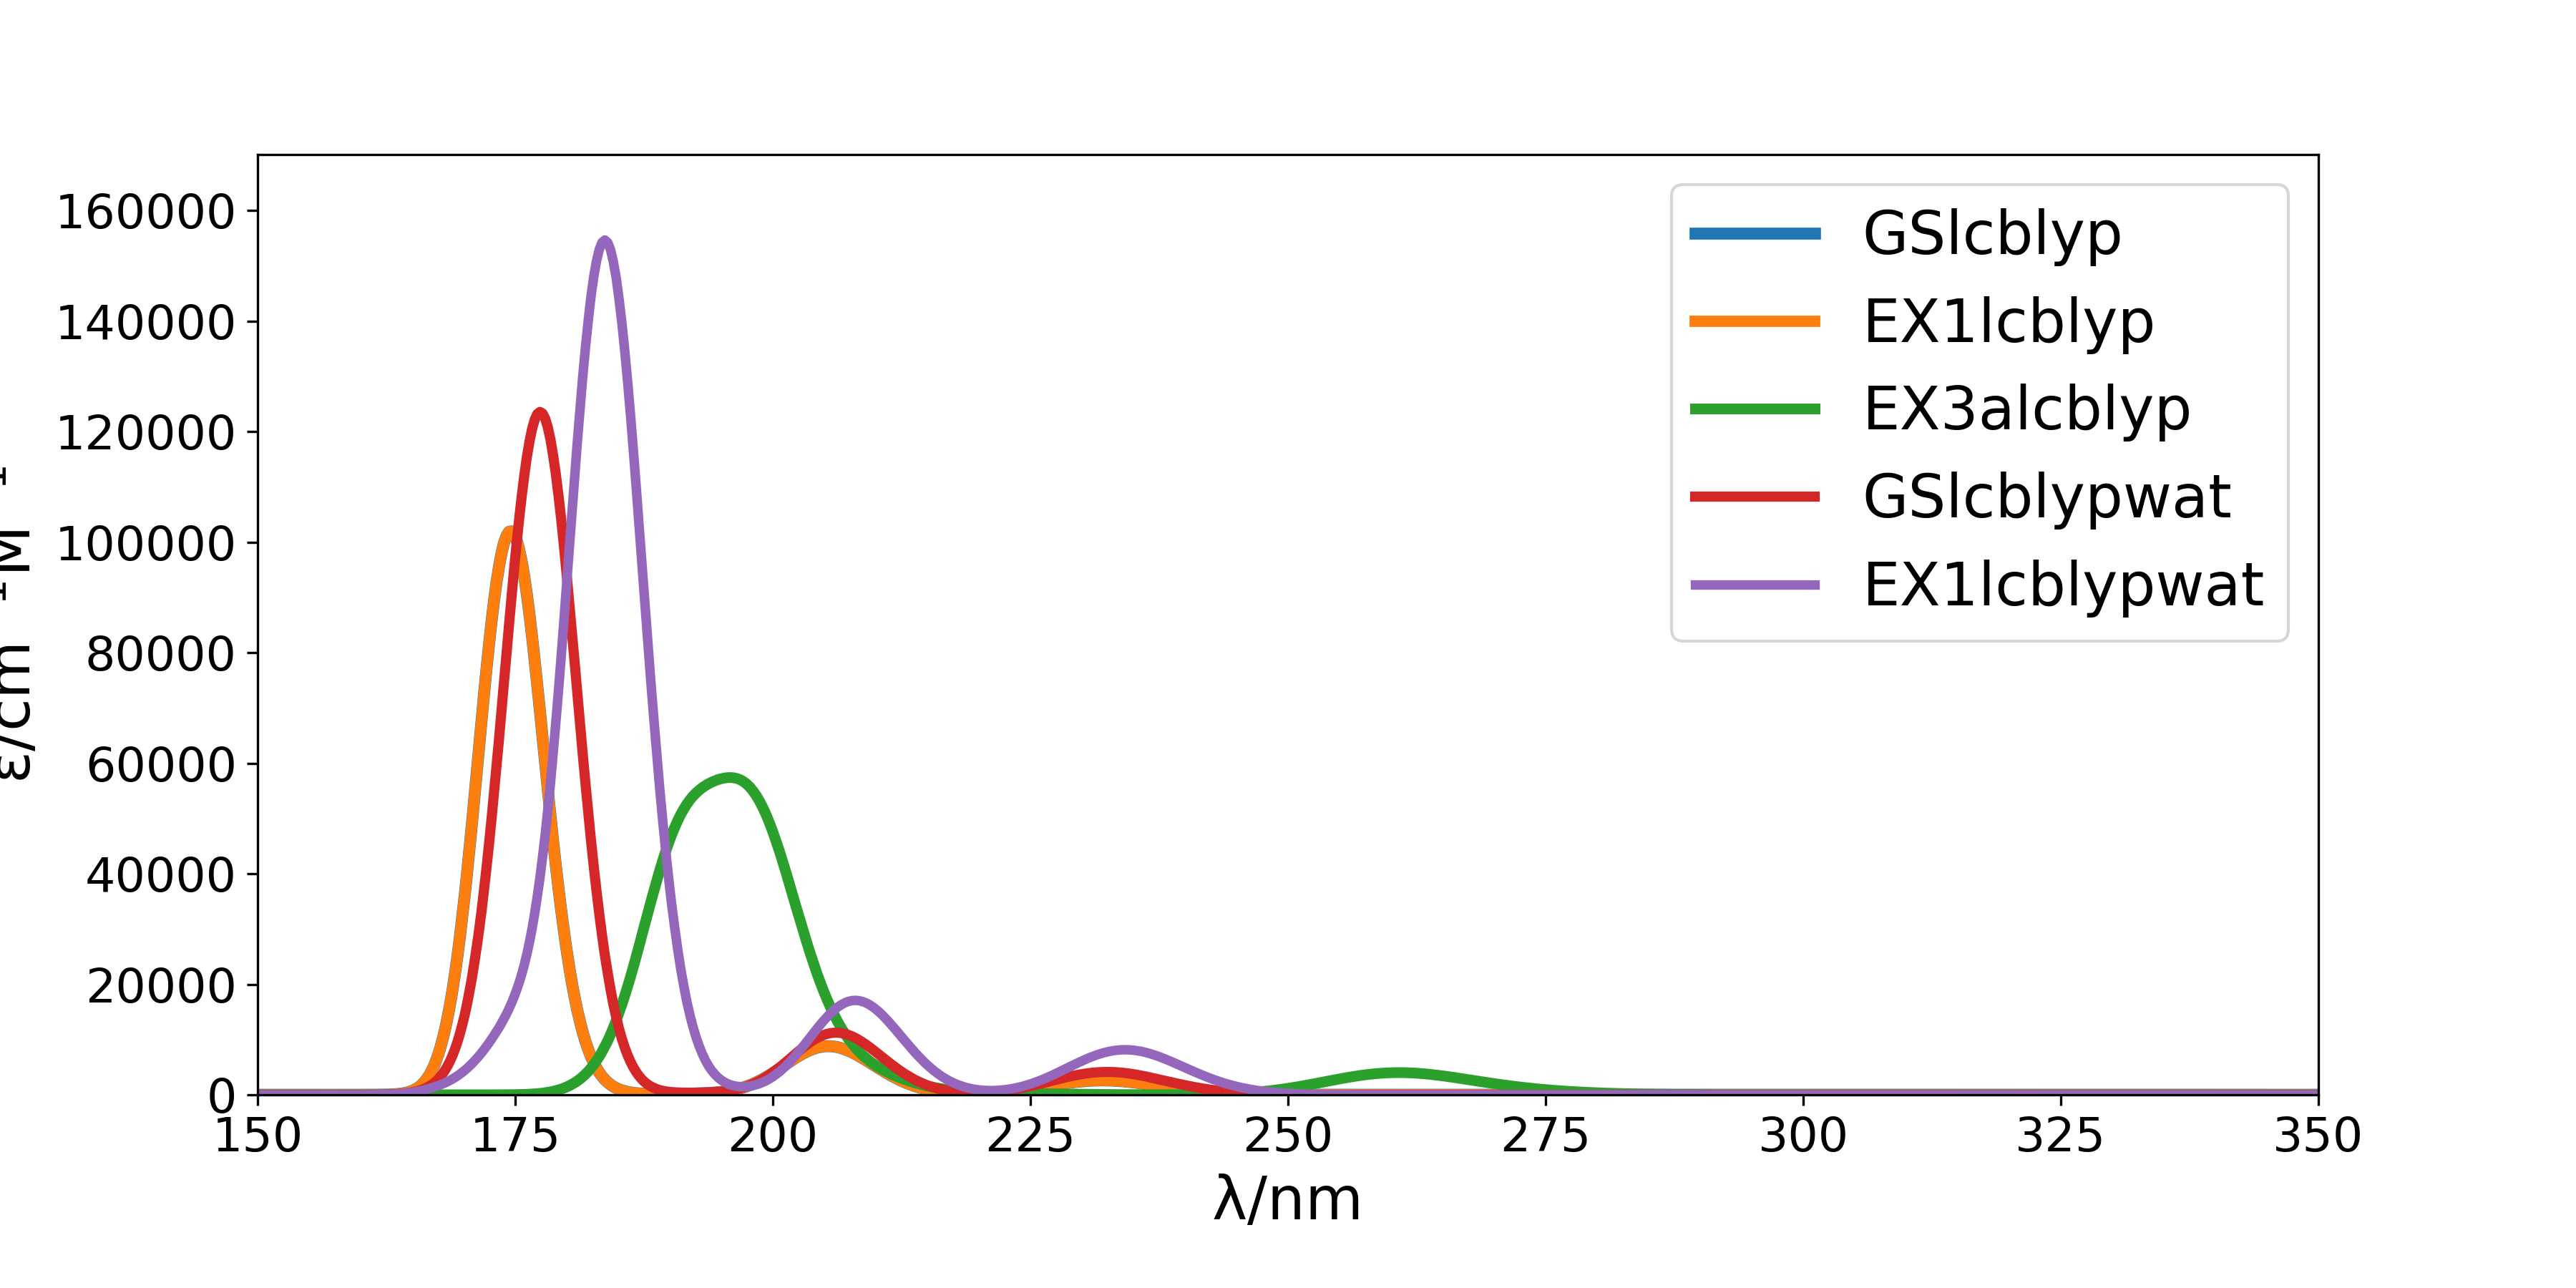
\includegraphics[width=\textwidth]{COMPlcblyp.png} 
	\caption{Comparison of different situations of tyrosine molecule calculated by lcblyp level of theory.}
	\label{COMPlcblyp}
\end{figure}

EPR: g = [1.94947   2.00212   2.00889]
 
 RMSD between optimized structure in ground state and in the first excited state, was measured to be 0.323.
 OH bond length of the phenol in the ground state optimized structure: 0.9669 A
 OH bond length of the phenol in the first excited state optimized structure: 0.9702 A
 OH bond length of the phenol in the first excited state optimized structure within water: 0.9770 A
 

%%%Table1
\begin{table}
	\small
	\caption{\ Impact of neighbors on magnetic parameters of radicals}
	\label{Dipole}
	\begin{tabular*}{\textwidth}{@{\extracolsep{\fill}}llll}
		\hline
		Dipole Moment (debye) & \ B3LYP  & \ LC-BLYP & \ CAM-B3LYP  \\
		\hline
		ground state   & 2.2156  &  2.5091  &  2.3384  \\
		ground state in PCM & 2.8769  &  3.2045  &  3.0148  \\
		ground state in H2O less than 3 A   & -  &  -  &  - \\
		1st excited state & 9.2362  &  2.4181  &  2.1943 \\
		1st excited in PCM & 3.0259  &   3.0479  &  2.8076 \\
		1st excited in H2O less than 3 A   & 5.5827  &  4.6990  &  4.8819 \\
		\hline
	\end{tabular*}
\end{table}


%%%Table2
\begin{table}
	\small
	\caption{\ Impact of neighbors on magnetic parameters of radicals}
	\label{SCFEnergy}
	\begin{tabular*}{\textwidth}{@{\extracolsep{\fill}}llll}
		\hline
		Energy (AU) & \ B3LYP  & \ LC-BLYP & \ CAM-B3LYP  \\
		\hline
		ground state   &  -837.99970  &  -835.87431  &  -837.61723 \\
		ground state in PCM & -838.01880  &  -835.89521  &  -837.63704  \\
		ground state in H2O less than 3 A   & -  &  -  &  - \\
		1st excited state & -837.99970  &  -835.87431  &  -837.61723\\
		1st excited in PCM & -838.01880 &   -835.89521  &  -837.63704 \\
		1st excited in H2O less than 3 A   & -2158.12866  &  -2153.56987  &  -2157.30960 \\
		\hline
	\end{tabular*}
\end{table}


\section{Conclusions}
Due to the proportional response of the EPR signal of \(\alpha\)-keratin to the absorbed dose, fingernail has been considered as a biodosimeter. However, the most challenging factor to consider while using fingernail EPR dosimetry is the presence of other types of signals other than the desired RIS. Here, we provided a qualitative analysis of the RIS radicals, in order to better develop methods for removing the MIS interference from the spectra and improving the accuracy of the measurements.


In order to do so, we considered three categories of radicals that might be produced in  \(\alpha\)-keratin sequence via reduction-oxidation processes. Moreover, regarding different cites of the probable radical species in keratin sequence, the right and left amino acids in the neighborhood of each case were also considered. Investigation of electronic structure in these quasi-closed-shell systems showed the SOMO-HOMO inversion which is typical organic molecules. Furthermore, we demonstrated that the SOMO-HOMO gap is proportional to spin localization.


Subsequently, we applied an MD simulation on the  \(\alpha\)-keratin in order to obtain the broadening ratio of  EPR spectrum due to the system's dynamics. The calculated quantity was then used in EasySpin package for spectra simulation. Also, it was indicated that different neighbors of the radical, doesn't play a significant role in signal position, and their effect is in the order of spectrum broadening.


The reliability of this method has been partly demonstrated by comparing the calculated parameters, with computational as well as experimental results, in literature. Through the analysis of the EPR signal of \(\alpha\)-keratin and underlying radicals, support is provided for the assignment of the RIS of low dose irradiation as a tyrosyl phenoxyl radical. While in high dose irradiation, the RSO radical is responsible for the originated RIS.










\section{References}

\subsection{References cited in the text}




\subsection{The list of references}

In the reference list, give the authors' names in the form in which they appear on the title page of the cited work. For names in the west European tradition, retain the order that puts the family name last (e.g. John J. Doe, not Doe, John J.). List all authors' names in the reference list, even in cases where there are three or more authors and where the preceding reference has the same author list. The following list shows some sample references prepared in Taylor \& Francis Reference Style O.

\begin{thebibliography}{99}

\bibitem{OpticalStimulated}
\bibitem{sebetic2008}
\bibitem{CoiledCoils}
\bibitem{KeratinStructure}
\bibitem{marciniak2016epr}
\bibitem{EPRofNail}
\bibitem{KeratinStructure}
\bibitem{Trompier2014}
\bibitem{EPR}
\bibitem{Symon1982}
\bibitem{EPRbiodosimetry}
\bibitem{Pailthorpe1972ESRACIDS}
\bibitem{1987-SulphurA-keratins}
\bibitem{Black2010ExRadicals}
\bibitem{Tipikin2016PossibleCalculations}
\bibitem{Dunlop1965}
\bibitem{GROVES2018}
\bibitem{Iikura2001}
\bibitem{neese2018software}
\end{thebibliography}
\bigskip

\begin{verbatim}
\begin{thebibliography}{99}

\bibitem{YF73}%1
G. Young and R.E. Funderlic, J. Appl. Phys. \textbf{44}, 5151 (1973).

\bibitem{NIST}%2
National Institutes of Standards and Technology, Physics Laboratory,
 Physical Reference Base.
 $<$http://physics.nist.gov./PhysRefData/contents.html$>$.

\bibitem{MBG69-74}%3
H. Massey, E. Burhop and H. Gilbody, editors, \emph{Electronic and
 Ionic Phenomena}, 5 vols. (Clarendon Press, Oxford, 1969--74).

\bibitem{Mar94}%4
J.E. Marsden and T.S. Ratiu, \emph{Introduction to Mechanics and
 Symmetry} (Springer, New York, 1994).

\bibitem{Lev77}%5
M.D. Levenson, Phys Today \textbf{30} (5), 44--49 (1977).

\bibitem{Tay66}%6
H.W. Taylor, J. Chem. Soc. \textbf{1966}, 411.

\bibitem{Koz73}%7
V. Kozub, Fiz. Tekh. Poluprovodn. \textbf{9}, 2284 (1975) [Sov. Phys.
 Semicond. 9, 1479 (1976)].

\bibitem{Bir71}%8
L.S. Birks, \emph{Electron Probe Microanalysis}, 2nd ed. (Wiley,
 New York, 1971), p.~40.

\bibitem{Ed72}%9
D.K. Edwards, in \emph{Proceedings of the 1972 Heat Transfer and
 Fluid Mechanics Institute}, edited by Raymond~B. Landis and Gary~J.
 Hordemann (Stanford University, Stanford, CA, 1972), pp. 71--72.

\bibitem{Tho73}%10
W.J. Thompson and D.R. Albert, US Patent No. 7,430,020 (3 March 1975).

\bibitem{Mos66}%11
J. Moskowitz, presented at the Midwest Conference on Theoretical
 Physics, Indiana University, Bloomington, IN, 1966 (unpublished).

\bibitem{Mik26}%12
R.C. Mikkelson (private communication).

\bibitem{Swa03}%13
R.T. Swan and C.M. Pitman, Saclay Report No. CEA-R 3147, 1957
 (unpublished).

\bibitem{Dan65}%14
J.B. Danda, Ph.~D. thesis,  Harvard University, 1965.

\bibitem{Nak73}%15
Y. Nakayama and S. Akita, New J. Phys. \textbf{5}, 128 (2003).
 $<$http://ej.iop.org/links/57/Hd+yfNDozFMnm2H8QoyUKA/njp3\_1\_128.pdf$>$.

\bibitem{HL74}%16
\emph{Technology: Catastrophe or Commitment?}, film produced by
 Hobel--Leiterman productions, Toronto (distributed by Document
 Associates, Inc., 880 Third Ave., New York, NY 10022; released 1974),
 16 mm, color, 24 min.

\bibitem{Bri72}%17
N.R. Briggs, computer code \textsc{crux} (Bell Laboratories, Murray
 Hill, NJ, 1972).

\bibitem{Zan03}%18
F. Zantow, O. Kaczmarek, F. Karsch, P. Petreczky, preprint,
 hep-lat/0301015 (2003).
 $<$http://www.thphys.uni.heidelberg.de/hep-lat/0301.html$>$.

\bibitem{Rid99}%19
W. Riddle and H. Lee, in \emph{Biomedical Uses of Radiation}, edited
 by W.R. Hendee (Wiley-VCH, Weinheim, Germany, 1999).

\bibitem{Gil75}%20a
T.L. Gilbert, Phys. Rev. B \textbf{12}, 2111 (1975).

\bibitem{Gil74}%20b
T.L. Gilbert, J. Chem. Phys. \textbf{60}, 3835 (1974).

\end{thebibliography}
\end{verbatim}
\bigskip
\noindent Each entry takes the form:
\begin{verbatim}
\bibitem{key}%n Bibliography entry
\end{verbatim}
where `\texttt{key}' is the tag that is to be used as an argument for the \verb"\cite{}" commands in the text of the article and `\texttt{Bibliography entry}' is the material that is to appear in the list of references, suitably formatted. The commands
\begin{verbatim}
\usepackage[numbers,sort&compress,merge]{natbib}
\bibpunct[, ]{[}{]}{,}{n}{,}{,}
\renewcommand\bibfont{\fontsize{10}{12}\selectfont}
\end{verbatim}
need to be included in the preamble of your .tex file in order to generate the citations and bibliography as described above.

Instead of typing the bibliography by hand, you may prefer to create the list of references using a \textsc{Bib}\TeX\ database. The \texttt{tfo.bst} file needs to be in your working folder or an appropriate directory, and the lines
\begin{verbatim}
\bibliographystyle{tfo}
\bibliography{interacttfosample}
\end{verbatim}
included where the list of references is to appear, where \texttt{tfo.bst} is the name of the \textsc{Bib}\TeX\ bibliography style file for Taylor \& Francis Reference Style O and \texttt{interacttfosample.bib} is the bibliographic database included with the \textsf{Interact}-TFO \LaTeX\ bundle (to be replaced with the name of your own .bib file). \LaTeX/\textsc{Bib}\TeX\ will extract from your .bib file only those references that are cited in your .tex file and list them in the References section.

Please include a copy of your .bib file and/or the final generated .bbl file among your source files if your .tex file does not contain a reference list in a \texttt{thebibliography} environment.



\end{document}
